\documentclass{assignment}

\usepackage{hyperref}

\begin{document}

% \title{CE CoP Python Workshop - VS Code Setup}




\assignmentTitle{CE CoP Python Workshop}{Jupyter Notebooks Setup}


Jupyter (formerly IPython Notebook) is an open-source project that lets you easily combine Markdown text and executable Python source code on one canvas called a notebook. All of the workshop's modules will be distributed via this files, setting up the environment will be vital to continue from this point on. In case anyone is stalled here, please do not hesitate to ask for help to the \href{mailto:computer.eng.cop.core.team@intel.com}{CE CoP core team}.

\section{Intel Devcloud Setup}

The Intel Devcloud provides a strightforward way to create and use Jupyter Notebooks with no extra steps required to setup an environment. Once you have the access to the Intel Devcloud that is everything you need to start working on it.

\subsection{Importing the files into the Devcloud}

In order to have the files as part of the devcloud, the following steps will be required:

\begin{enumerate}
    \item Unzip the .ipynb files provided for this workshop in a known location. 
    \item Go to \href{https://jupyter.oneapi.devcloud.intel.com/hub/login?next=%2Fhub%2F}{https://jupyter.oneapi.devcloud.intel.com/hub/login?next=\%2Fhub\%2F}.
    \item Press ``Click Here to Sign In" button.
    \item Provide your intel’s email and press “Continue” button 
    \item { 
        Select the file browser view by clicking the folder icon on the left as shown in Figure \ref{fig:import_0}.
        \begin{figure}[h]
         \centering 
            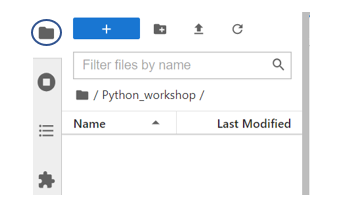
\includegraphics[width=6cm]{assets/intel_devcloud_login.png}
            \caption{File browser}
            \label{fig:import_0}
        \end{figure}
    }

    \item {
        Select ``New Folder" option as presented in Figure \ref{fig:import_1}.
        \begin{figure}[h]
         \centering 
            
\includegraphics[width=6cm]{assets/intel_devcloud_new_folder.png}
            \caption{New folder creation}
            \label{fig:import_1}
        \end{figure}
    }
    \item Enter ``Python\_workshop" as folder’s name.
    \item Open the ``Python\_workshop" folder by double clicking over its name.
    \item {
        Select ``Upload Files" option. See Figure \ref{fig:import_2} for reference.
        \begin{figure}[h]
         \centering 
            
\includegraphics[width=6cm]{assets/intel_devcloud_upload.png}
            \caption{Uploading the files}
            \label{fig:import_2}
        \end{figure}        
    }
    \item Select all the .ipynb files and press the ``Open" button.
    \item Open the files by double clicking over its name.
\end{enumerate}

\newpage

\section{VS Code Setup}
% \lstinputlisting[language=C++]{assets/test.cpp}

Visual Studio Code supports working with Jupyter Notebooks natively, and through Python code files. To work with Python in Jupyter Notebooks, you must activate an Anaconda environment in VS Code, or another Python environment in which you've installed the Jupyter package. 

\subsection{Automatically setting up your environment}

VS Code can handle the installation of those packages automatically. Once you request to create a new file and it does not know how to deal with it, it will suggest to install what is required to execute that specific file extension. In Figure \ref{fig:new_file_0} you will see where to create a new file.

\begin{figure}[h]
 \centering 
    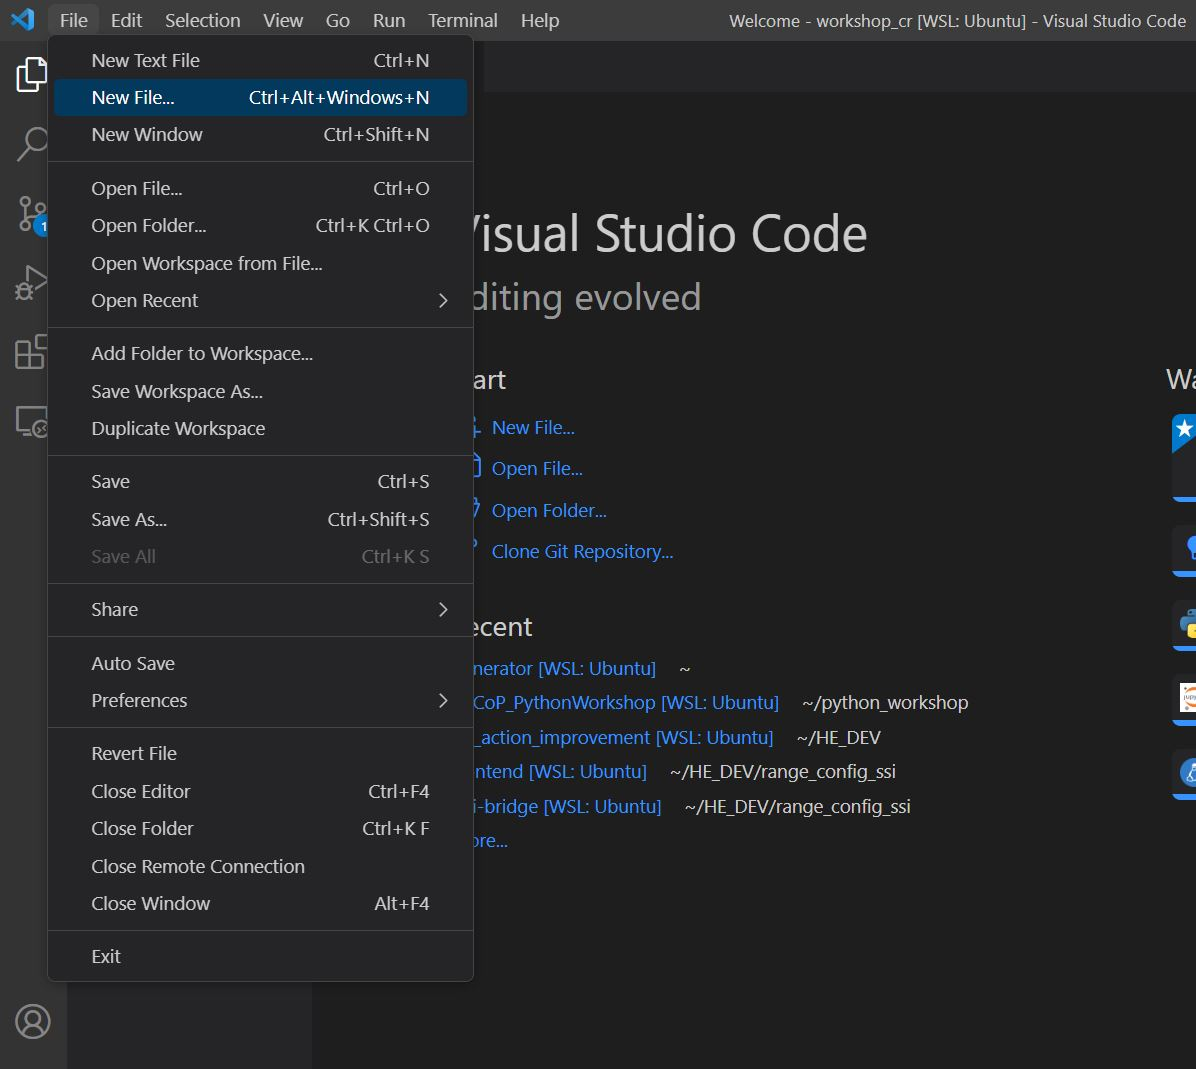
\includegraphics[width=11cm]{assets/vs_code_new_file.JPG}
    \caption{Creating a new file}
    \label{fig:new_file_0}
\end{figure}

\newpage

Then you will require to select the file extension for VS Code to trigger the automatic setup. In Figure \ref{fig:new_file_1}, once you type ``Jup" to look for the file extension, it will suggest the type you are looking for.

\begin{figure}[h]
 \centering 
    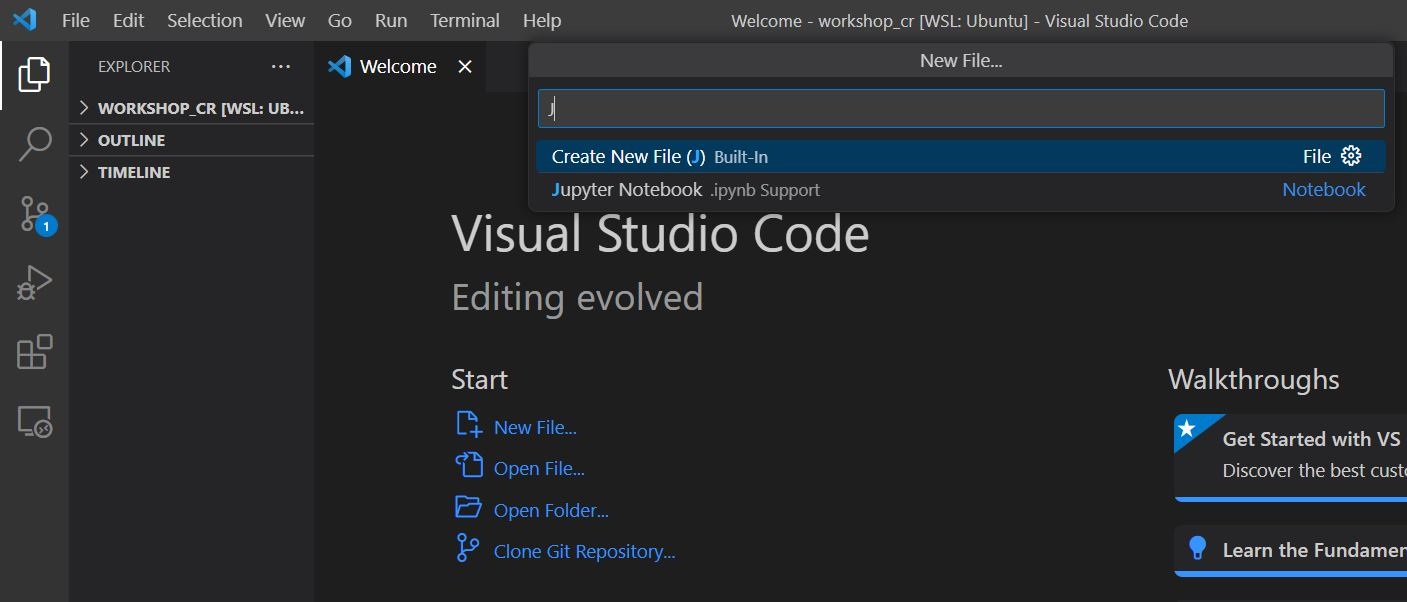
\includegraphics[width=11cm]{assets/vs_code_jupyter_notebook.JPG}
    \caption{Picking the file extension}
    \label{fig:new_file_1}
\end{figure}


As soon as you click on the type, an empty file will be created such as the one presented in Figure \ref{fig:new_file_2}.

\begin{figure}[h]
 \centering 
    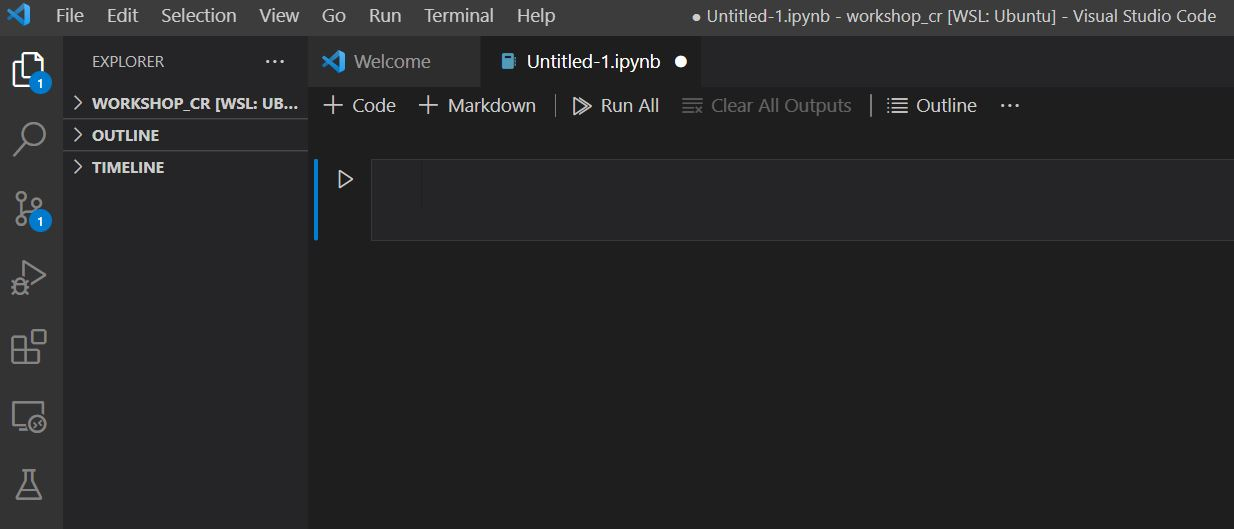
\includegraphics[width=11cm]{assets/vs_code_empty_file.JPG}
    \caption{Empty file created}
    \label{fig:new_file_2}
\end{figure}

There are a couple places where to execute the file, but whenever you hit the play button in a similar fashion than in Figure \ref{fig:new_file_3}.a, VS Code will automatically try to execute the code, if it does not have an interpreter an the required packages, it will suggest you to proceed with the installations as in Figure \ref{fig:new_file_3}.b.

\begin{figure}[h]
 \centering
 \begin{minipage}{12cm}
        (a)
        \centering
        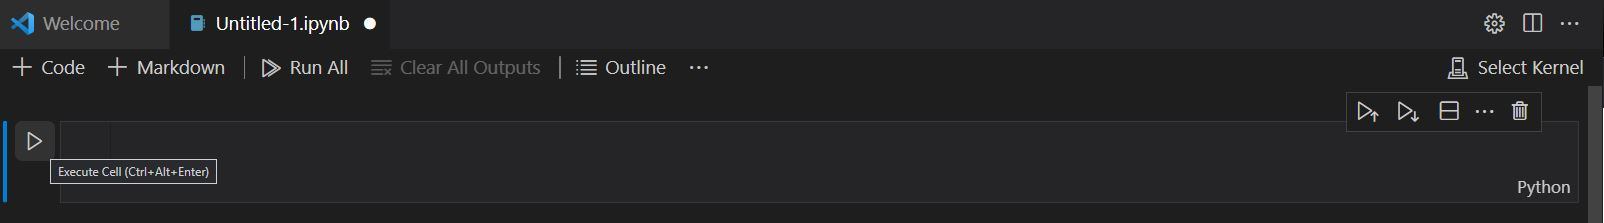
\includegraphics[width=11cm]{assets/vs_code_empty_file_run_button.JPG}
 \end{minipage}
 \begin{minipage}{12cm}
    (b)
    \centering
        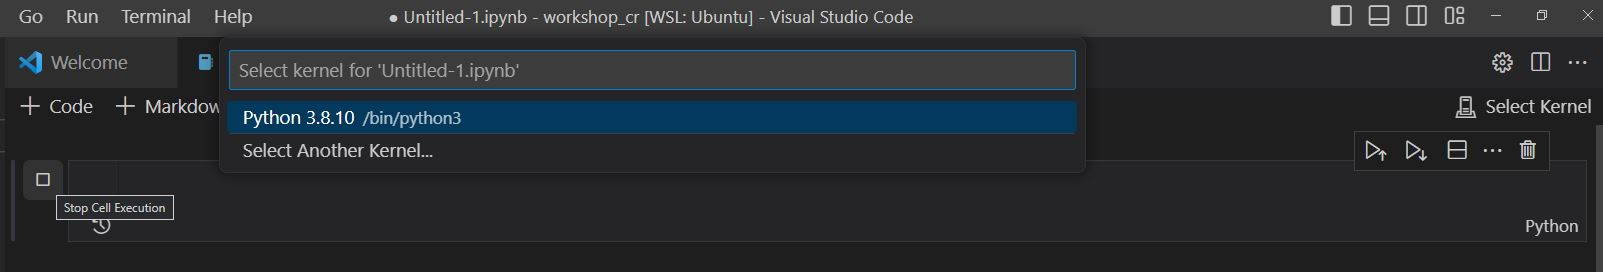
\includegraphics[width=11cm]{assets/vs_code_empty_file_run_button_hit.JPG}
 \end{minipage}
 \caption{Play button on a new file}
 \label{fig:new_file_3}
\end{figure}
\newpage
\subsection{Manual installation/setup}

To select an environment, use the Python: Select Interpreter command from the Command Palette (\textcolor{cyan}{Ctrl+Shift+P}). Once the appropriate environment is activated, you can create and open a Jupyter Notebook, connect to a remote Jupyter server for running code cells, and export a Jupyter Notebook as a Python file.

In case you want to have a better understanding on how this is managed, please visit \href{https://code.visualstudio.com/docs/datascience/jupyter-notebooks}{Jupyter Notebooks in VS Code}.

\subsection{Importing the files into VS Code}

Having the files placed into VS Code is quite simple, please follow these steps:

\begin{enumerate}
    \item Unzip the .ipynb files provided for this workshop in a known location.
    \item Have VS Code opened.
    \item {
        As shown in Figure \ref{fig:vsc_import_0}, hit on ``Open Folder...".
        \begin{figure}[h]
         \centering 
            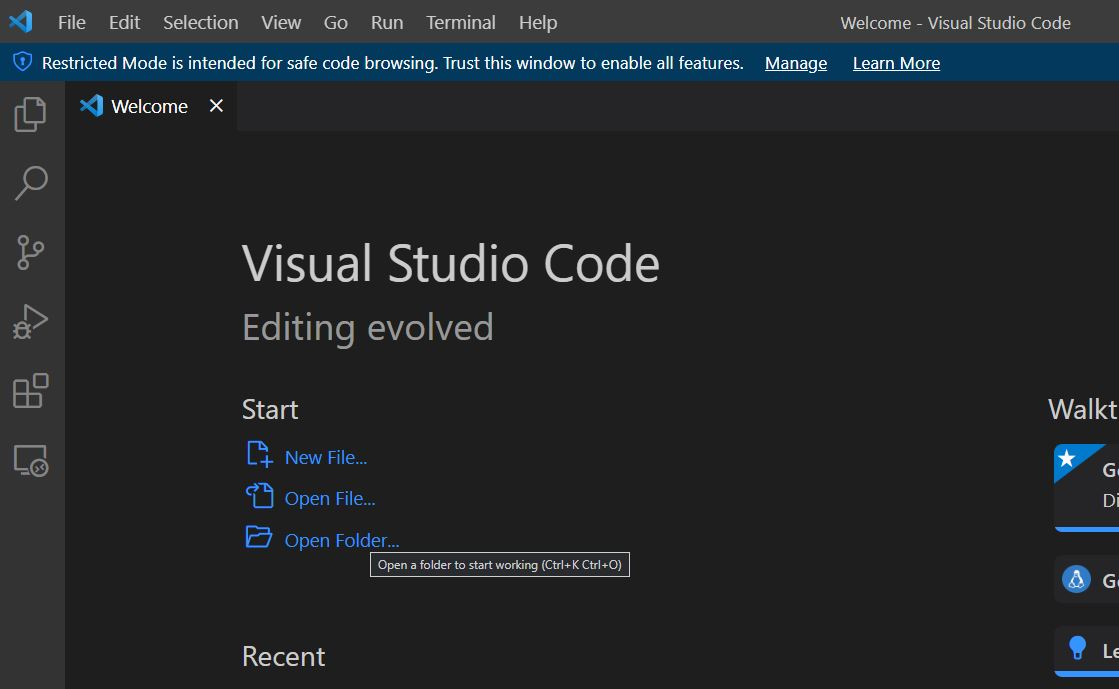
\includegraphics[width=12cm]{assets/vs_code_open_folder.JPG}
            \caption{Importing the workshop directory.}
            \label{fig:vsc_import_0}
        \end{figure}
    }
    \newpage
    \item {
        On the ``Open Folder" view, select the known path where the files were extracted. Figure \ref{fig:vsc_import_1} is a reference.
        \begin{figure}[h]
         \centering 
            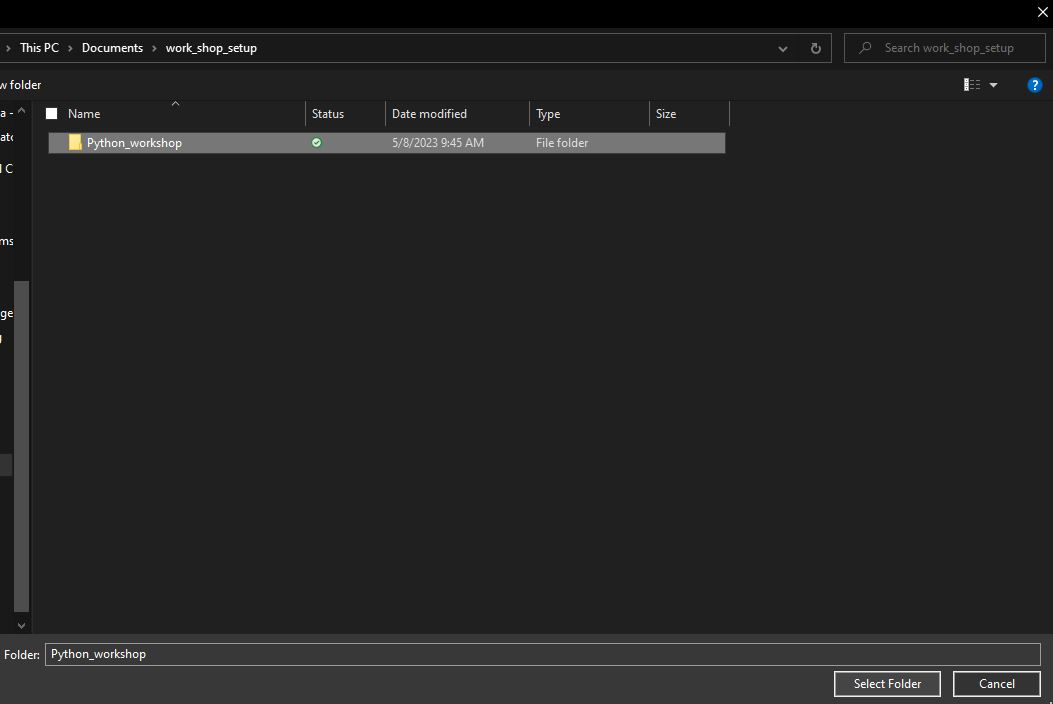
\includegraphics[width=11cm]{assets/vs_code_select_folder.JPG}
            \caption{Opening files.}
            \label{fig:vsc_import_1}
        \end{figure}        
    }
    \item {
        Click on any file that has been imported to open it. See Figure \ref{fig:vsc_import_2}.
        \begin{figure}[h]
         \centering 
            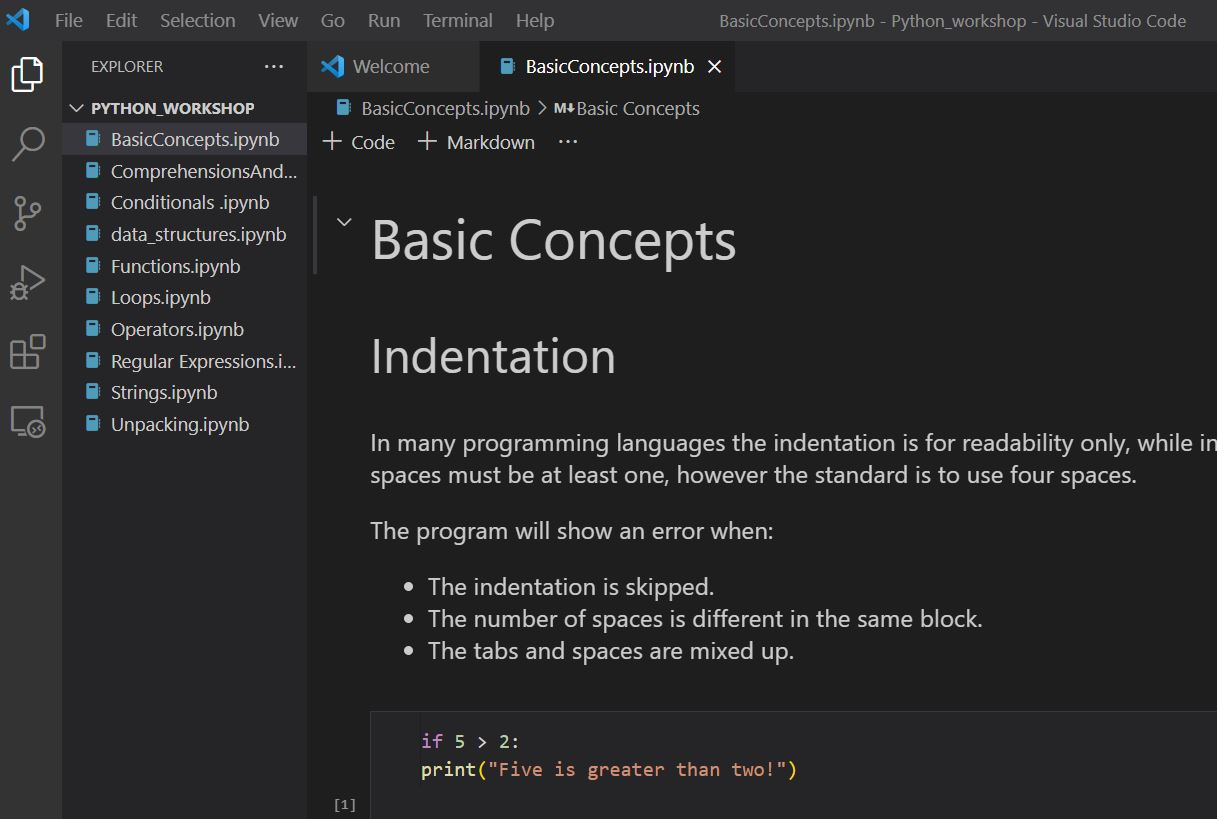
\includegraphics[width=11cm]{assets/vs_code_opened_file.JPG}
            \caption{Opening files.}
            \label{fig:vsc_import_2}
        \end{figure}
    }
    
\end{enumerate}

\end{document}
